\documentclass{beamer}

\mode<presentation>
{
\usetheme{Madrid}
}

\usepackage{graphics, graphicx}
\usepackage{booktabs}
\DeclareGraphicsExtensions{.pdf,.png,.jpg,.gif}

\title{Linux Beginner Guide}

\author{Jaewoong Lee}

\institute[UNIST]
{
	Ulsan National Institute of Science and Technology
	\medskip
	\newline
	\textit{jwlee230@unist.ac.kr}
}

\date{\today}

\begin{document}
	\begin{frame}
		\titlepage
	\end{frame}

	\begin{frame}
		\frametitle{Introduction}
		
		In this guide, I assume that followings are already installed:
		\begin{enumerate}
			\item Ubuntu 16.04.2 or Higher
			\item ZSH 5.0.2 or Higher
			\item VIM 8.1 or Higher
			\item We will connect to server via SSH
		\end{enumerate}

		With this guide, you can use and understand Linux system. \\
		Also, this guide includes as little information about operating system as possible. If you find some fault in the strict sense of the word, that means you are not \textbf{beginner}. 
	\end{frame}

	\begin{frame}
		\frametitle{Overview}
		\tableofcontents
	\end{frame}

	\section{Linux?}
	
	\begin{frame}
		\frametitle{Linux?}
		\begin{figure}[h!]
			\centering
			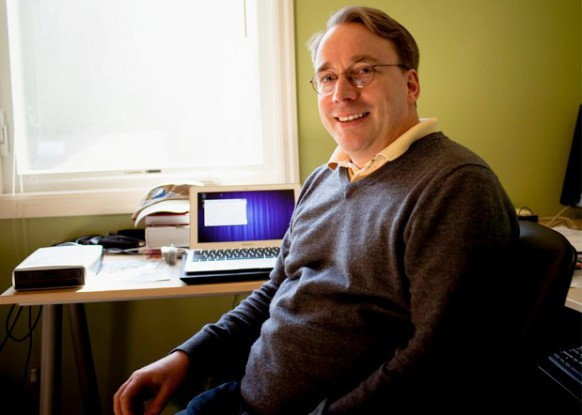
\includegraphics[width=0.4 \linewidth]{figures/linus.jpg}
			\caption{Linus Torvalds, Inventor of Linux}
		\end{figure}
	
		Linux is one of the most famous OS as Windows and macOS. \\
		Linux is open-source project. \\
		Android, OS for mobile, is based on Linux. 
	\end{frame}

	\begin{frame}
		\frametitle{Ubuntu?}
		\begin{figure}[h!]
			\centering
			
\includegraphics[width=0.3 \linewidth]{figures/ubuntu.jpg}
			\caption{Logo of Ubuntu}
		\end{figure}
		Ubuntu is an OS which is based on Linux. \\
		Ubuntu is the best OS in Linux-like OS, because of convenience of its installation and usage.
	\end{frame}
	
	\section{Basic Linux Command}
	
	\begin{frame}
		\frametitle{Where we start}
		\begin{figure}[h!]
			\centering
			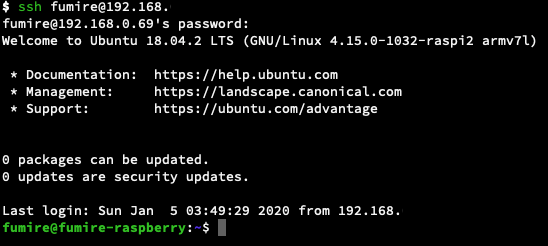
\includegraphics[width=0.5 \linewidth]{figures/1.png}
			\caption{Here is where we start}
		\end{figure}
	
		After you connect to server via SSH, you can see like this. \\
		Here is where we start! \\
		\textit{fumire} will be user name, and \textit{fumire-raspberry} will be server name. 
	\end{frame}

	\begin{frame}
		\frametitle{pwd}
		\begin{figure}[h!]
			\centering
			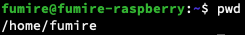
\includegraphics[width=0.5 \linewidth]{figures/2.png}
			\caption{Result of \textit{pwd} Command}
		\end{figure}
		\textit{pwd} is abbr. of "Print Working Directory". \\
		You can see where you are with \textit{pwd} command. \\
		Also, "/home/username" is your \textit{home folder}, a.k.a. '$\sim$'.
	\end{frame}

	\begin{frame}
		\frametitle{ls}
		\begin{figure}[h!]
			\centering
			
\includegraphics[width=0.7 \linewidth]{figures/3.png}
			\caption{Result of \textit{ls} Command}
		\end{figure}
	
		\textit{ls} stands for "List". \\
		\textit{ls} command lists current directory contents. \\
		If current directory is empty, the result will be nothing. 
	\end{frame}

	\begin{frame}
		\frametitle{Configuration}
		However, you have not completed configuration. Therefore, finish settings with following command:
		\begin{example}
			\$ git clone https://github.com/Fumire/.dotfiles.git \\
			\$ cd .dotfiles \\
			\$ make \\
			\$ chsh -s /usr/bin/zsh
		\end{example}
		Note that you should input command only after '\$'. \\
		After executing commands, you should restart your shell. 
	\end{frame}

	\begin{frame}
		\frametitle{Configuration \textit{(Cont.)}}
		\begin{figure}[h!]
			\centering
			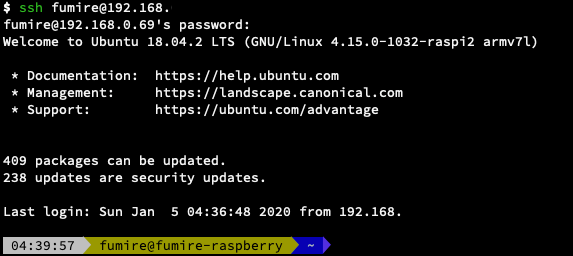
\includegraphics[width=0.7 \linewidth]{figures/4.png}
			\caption{ZSH}
		\end{figure}
	
		With successful configuration, you can see like this. 
	\end{frame}

	\begin{frame}
		\frametitle{Tip!}
		\begin{figure}[h!]
			\centering
			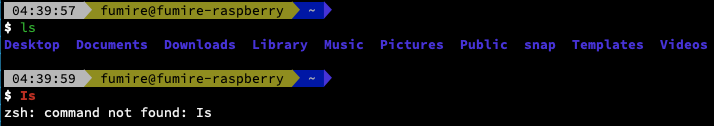
\includegraphics[width=0.7 \linewidth]{figures/5.png}
			\caption{Right Command vs. Wrong Command}
		\end{figure}
		
		You can easily know this command is right with ZSH as figure.  
	\end{frame}

	\begin{frame}
		\frametitle{mkdir}
		\textit{mkdir} stands for "Make Directory". \\
		You can make a directory which named 'test' as following: 
		\begin{example}
			\$ mkdir test \\
			or \\
			\$ md test \\
		\end{example}
		\textit{mkdir} returns nothing. Literally, \textit{mkdir} command only make directory. \\
		You can check that the directory has been made with \textit{ls} command. 
	\end{frame}

	\begin{frame}
		\frametitle{cd}
		\textit{cd} is abbr. of "Change Directory". \\
		You can change your working directory to 'test' as following:
		\begin{example}
			\$ pwd \\
			\$ cd test\\
			\$ pwd \\
		\end{example}
	
		Also, you can go your home folder at once with \textit{cd}, no matter where you are.
		\begin{figure}[h!]
			\centering
			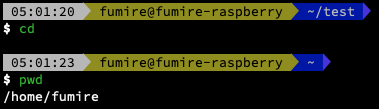
\includegraphics[width=0.7 \linewidth]{figures/6.png}
			\caption{\textit{cd} will guide you to home folder}
		\end{figure}
	\end{frame}

	\begin{frame}
		\frametitle{Tip!}
		If you hit "Tab" button, ZSH will give proper candidates. \\
		Following example shows what ZSH gives.
		\begin{figure}
			\centering
			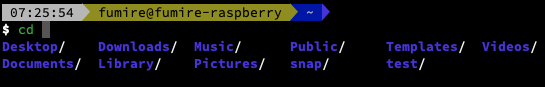
\includegraphics[width=0.7 \linewidth]{figures/10.png}
			\caption{Shortcut with Tab}
		\end{figure}
	\end{frame}

	\begin{frame}
		\frametitle{man and -$ $-help}
		You can get detailed information about command as following:
		\begin{example}
			\$ man ls \\
			and/or \\
			\$ ls -$ $-help
		\end{example}
		This guide will give simple information about Linux command. Hence, when you have curiosity about command, use these command.
	\end{frame}

	\begin{frame}
		\frametitle{Directory Structure}
		Try following commands:
		\begin{example}
			\$ cd test\\
			\$ ls -al
		\end{example}
		Then, you can see like this:
		\begin{figure}[h!]
			\centering
			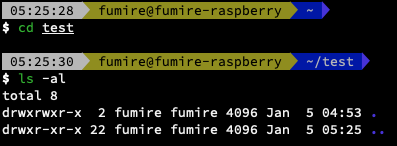
\includegraphics[width=0.3 \linewidth]{figures/7.png}
			\caption{Result of \textit{ls} command}
		\end{figure}
		All directory has '.' and '..', even though the directory is empty. \\
		'.' means current directory itself; and, '..' means parent directory.
	\end{frame}

	\begin{frame}
		\frametitle{touch}
		\textit{touch} command make new file or touch the file.
		
		Try following example:
		\begin{example}
			\$ cd \\
			\$ touch t \\
			\$ ls
		\end{example}
		
		Then, you can see that the file which name 't' has been made. 
	
		\begin{figure}[h!]
			\centering
			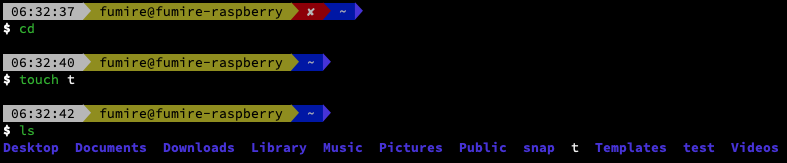
\includegraphics[width=0.5 \linewidth]{figures/8.png}
			\caption{Result of \textit{touch} Command}
		\end{figure}
	\end{frame}

	\begin{frame}
		\frametitle{mv}
		\textit{mv} command moves/renames file. \textit{mv} is used as:
		\begin{example}
			\$ mv SRC(source) DST(destination)
		\end{example}
		
		Try following commands: 
		\begin{example}
			\$ mv t tmp \\
			\$ ls \\
			\$ mv tmp test/ \\
			\$ ls
		\end{example}
	
		Then, you will realize that the file 'tmp' is gone. I hope that you already know where the file goes. :)
	\end{frame}

	\begin{frame}
		\frametitle{cp}
		\textit{cp} command copies SRC to DST. \textit{cp} is used as:
		\begin{example}
			\$ cp SRC DST
		\end{example}
	
		Try following commands:
		\begin{example}
			\$ cd $\sim$/test/ \\
			\$ ls \\
			\$ cp tmp tmp2 \\
			\$ ls
		\end{example}
		Then, you can realize that a new file 'tmp2' has been made. 
	\end{frame}

	\begin{frame}
		\frametitle{sudo}
		\textit{sudo} is abbr. of "Substitute User do"; but, many people know as "Super User do". \\

		\textit{sudo} allows a system administrator to delegate authority to give certain user the ability to run some command as another user.
		
		\begin{figure}[h!]
			\centering
			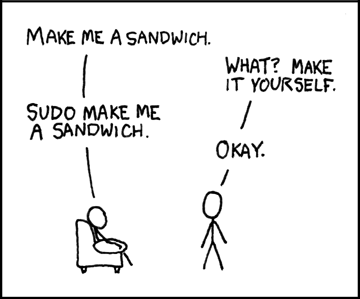
\includegraphics[width=0.3 \linewidth]{figures/sudo.png}
			\caption{XKCD: Sandwich}
		\end{figure}
	
		THINK what will happen after \textit{sudo} command!!
	\end{frame}

	\section{Edit File with VIM} 
	
	\begin{frame}
		\frametitle{Editor}
		There are three major editors in Linux.
		\begin{figure}[h!]
			\centering
			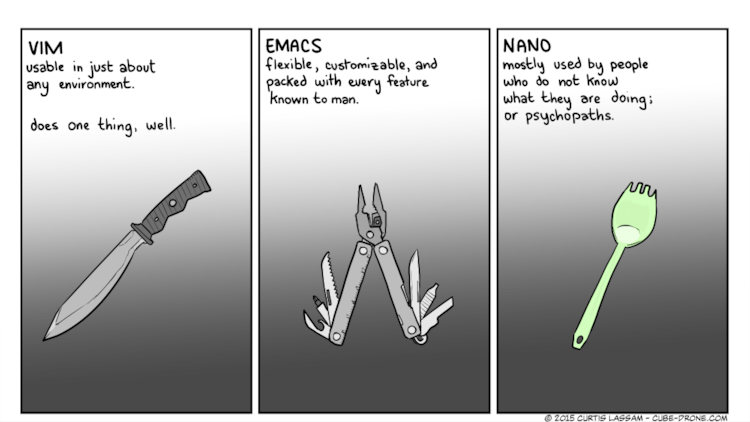
\includegraphics[width=0.7 \linewidth]{figures/editor.png}
			\caption{Descriptions of Editor}
		\end{figure}
		For this reason, this guide use VIM editor. 
	\end{frame}

	\begin{frame}
		\frametitle{Editor \textit{Cont.}}
		\begin{figure}[h!]
			\centering
			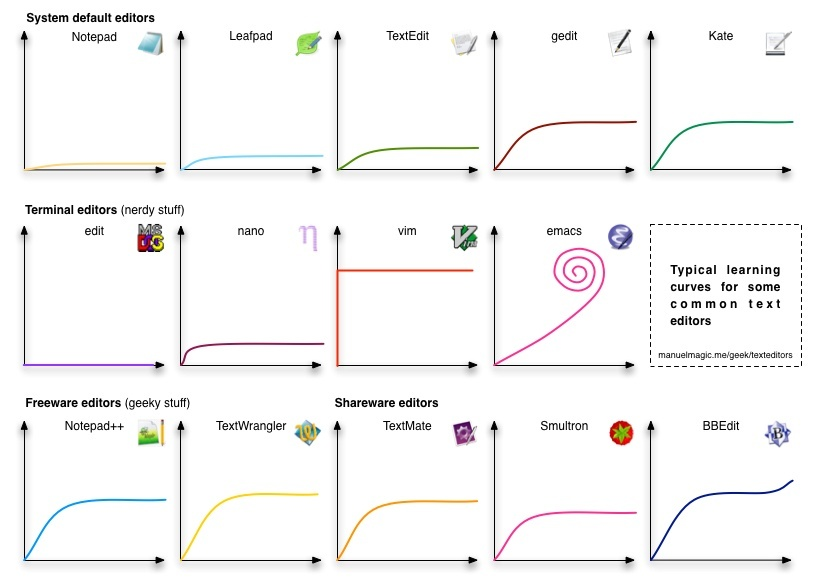
\includegraphics[width=0.7 \linewidth]{figures/curves.jpg}
			\caption{Learning Curves among Editors}
		\end{figure}
	\end{frame}

	\begin{frame}
		\frametitle{First Meet with VIM}
		With these commands, you can make/edit file.
		\begin{example}
			\$ vi tmp
		\end{example}
	
		If it is first time to open VIM, then you will see like this. 
		\begin{figure}[h!]
			\centering
			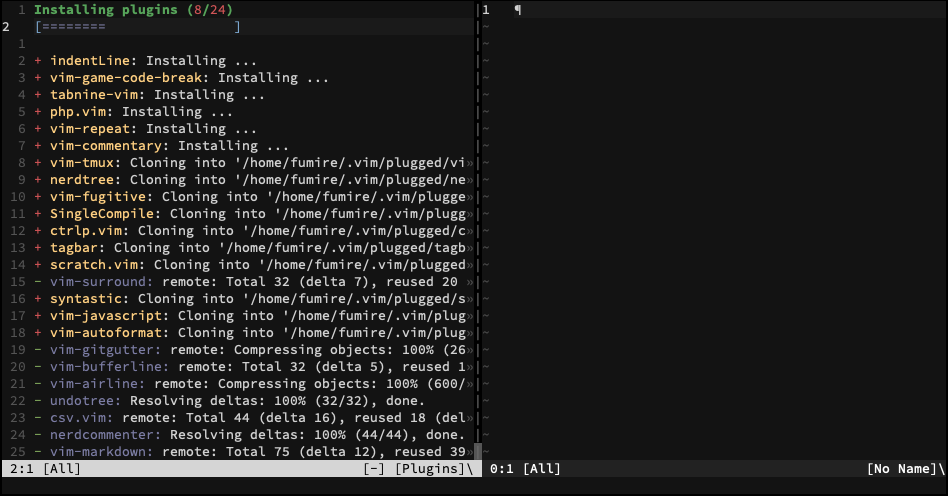
\includegraphics[width=0.5 \linewidth]{figures/9.png}
			\caption{First Time of VIM}
		\end{figure}
	\end{frame}

	\begin{frame}
		\frametitle{Modes of VIM}
		\begin{figure}[h!]
			\centering
			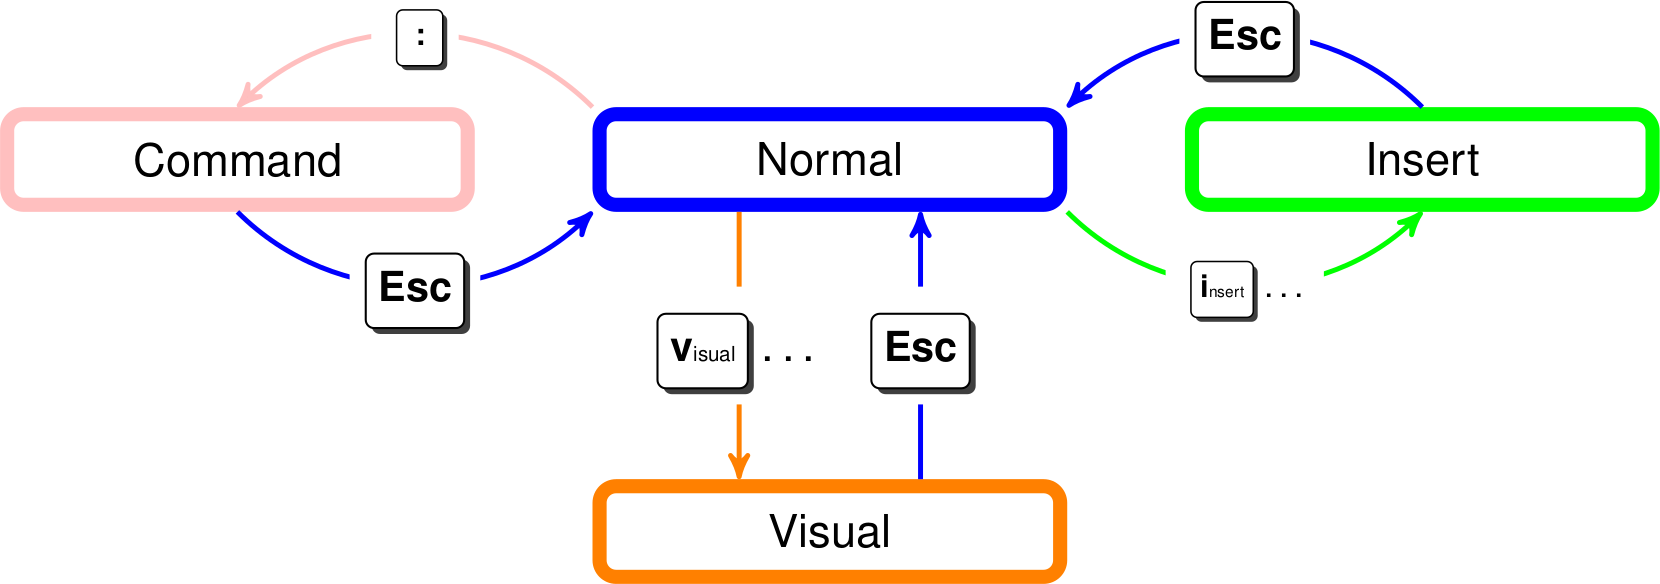
\includegraphics[width=0.7 \linewidth]{figures/modes.png}
			\caption{Three Modes in VIM}
		\end{figure}
	\end{frame}

	\begin{frame}
		\frametitle{How to Edit with VIM}
		Editing with VIM is following such steps:
		\begin{enumerate}
			\item Press 'i'
			\item Edit the file
			\item Press 'ESC'
			\item Enter ':w' which means \textit{write}
			\item Enter ':q' wihch means \textit{quit}
		\end{enumerate}
	\end{frame}

	\begin{frame}
		\frametitle{Plugin Setting (Optional)}
		You might see the error message because the plugin setting is not completed. To solve this, use following commands:
		\begin{example}
			\$ cd $\sim$/.vim/plugged/tabnine-vim/ \\
			\$ python3 install.py 
		\end{example}
		Then, all plugin acts properly without errors. 
	\end{frame}

	\section{IO Redirections}
	
	\begin{frame}
		\frametitle{cat}
		\textit{cat} stands for con\textbf{cat}enate. \textit{cat} command reads files, and writing them to standard output. \\
		Consider following example:
		\begin{example}
			\$ cd $\sim$/test/ \\
			\$ cat tmp 
		\end{example}
		You can see contents of file. 
	\end{frame}

	\begin{frame}
		\frametitle{Output to file}
		If you want redirect output to file, use following example:
		\begin{example}
			\$ cat tmp $>$ output
		\end{example}
		However, this method \textit{overwrites} the contents of file. \\
		If you want preserve the file contents, use following: 
		\begin{example}
			\$ cat tmp $>>$ output
		\end{example}
	\end{frame}

	\begin{frame}
		\frametitle{Output to file \textit{Cont.}}
		In some cases, you should divide standard output and standard error. \\
		In these cases, use following commands:
		\begin{example}
			\$ commands 1$>$ STDOUT 2$>$ STDERR
		\end{example}
	
		\begin{example}
			\$ cat tmp 1$>$ ex.stdout 2$>$ ex.stderr 
		\end{example}
	\end{frame}

	\begin{frame}
		\frametitle{more / less}
		\textit{more} and \textit{less} are commands for seeing the contents of file.
		Consider following examples:
		\begin{example}
			\$ more tmp
		\end{example}
	
		\begin{example}
			\$ less tmp
		\end{example}
	\end{frame}

	\begin{frame}
		\frametitle{Pipe}
		Use pipe ($|$) to indicate input as output of previous command.
		\begin{example}
			\$ command1 $|$ command2
		\end{example}
		The output of command 1 will be the input of command2. \\
		Consider following example: 
		\begin{example}
			\$ cat tmp $|$ less
		\end{example}
	\end{frame}
	
	\section{How to Download from Web}
	
	\section{User Permissions}
	
	\section{Process Control}
	
	\section{Process Control with SGE}

\end{document}